\documentclass[dvipsnames]{beamer}
\mode<presentation>{}
\usepackage[utf8]{inputenc}
\usepackage{amsmath, amssymb, amsfonts, amsthm, mathtools, mathrsfs}
\setbeamertemplate{theorems}[numbered]
\title{CS347M Take-home Quiz 3}
\author{Prasann Viswanathan}
\date{Spring Semester 2021-22}
\institute[IITB]{IIT Bombay}
\usetheme{Warsaw}
% \usecolortheme{beetle}
\hypersetup{colorlinks=true}
\addtobeamertemplate{footline}{\hypersetup{allcolors=.}}{}
\usepackage{parskip}
\usepackage{tcolorbox}

\usepackage{tikz}
\usetikzlibrary{decorations.markings}
\usetikzlibrary{arrows.meta}

\newcommand{\id}{\operatorname{id}}
\newcommand{\Res}{\operatorname{Res}}
% \renewcommand{\exp}{\operatorname{exp}}

\theoremstyle{definition}
\newtheorem{defn}{Definition}
\newtheorem{prop}{Proposition}
\newtheorem{thm}{Theorem}
\newtheorem{rem}{Remark}

\begin{document}
\tikzset{lab dis/.store in=\LabDis,
  lab dis=-0.4,
  ->-/.style args={at #1 with label #2}{decoration={
    markings,
    mark=at position #1 with {\arrow{>}; \node at (0,\LabDis) {#2};}},postaction={decorate}},
  -<-/.style args={at #1 with label #2}{decoration={
    markings,
    mark=at position #1 with {\arrow{<}; \node at (0,\LabDis)
    {#2};}},postaction={decorate}},
  -*-/.style args={at #1 with label #2}{decoration={
    markings,
    mark=at position #1 with {{\fill (0,0) circle (1.5pt);} \node at (0,\LabDis)
    {#2};}},postaction={decorate}},
  }
\begin{frame}
    \titlepage
\end{frame}

\begin{frame}{Cigarette Smokers Problem}
    The cigarette smokers problem is one of the classical problems. It was posed by Suhas Patil, who claimed it could be solved by semaphores. In this presentation I attempt to explain and implement the problem in code.
\end{frame}

\begin{frame}{Problem statement}
\begin{enumerate}
    \item Four threads are involved: an agent and three smokers. The smokers loop forever, first waiting for ingredients, then making and smoking cigarettes. 
    \item We assume that the agent has an infinite supply of all three distinct ingredients, and each smoker has an infinite supply of one of the ingredients.
    \item The agent repeatedly chooses two different ingredients at random and makes them available to the smokers. Depending on which ingredients are chosen, the smoker with the complementary ingredient should pick up both resources and proceed.
\end{enumerate}
\end{frame}

\begin{frame}{Restrictions}
To model a resource-management problem of operating systems in real situations, the following constraints are applied to the agent:
\begin{enumerate}
    \item  The agent is only allowed to communicate by signaling the availability of a resource using a condition variable or semaphore.
    \item The agent is not permitted to disclose resource availability in any other way; i.e., smokers cannot ask the agent what is available.
    \item The agent is not permitted to know anything about the resource needs of smokers; i.e., the agent cannot wakeup a smoker directly.
    \item Each time the agent makes two resources available, it must wait on a condition variable for a smoker to smoke before it can make any additional resources available.
\end{enumerate}
\end{frame}

\begin{frame}{Crux of the question}
When the agent makes two items available, \textbf{every smoker} thread can use at least one of them, but \textbf{only one} can use both. For example, if the agent makes paper and matches available, both the paper and the matches smokers want one of these, but neither will be able to smoke because neither has tobacco. But, if either of them does wake up and consume a resource, that will prevent the tobacco thread from begin able to smoke and thus also prevent the agent from waking up to deliver additional resources. If this happens, the system is deadlocked. This is the idea to give wrong implementations as well.
\end{frame}

\begin{frame}{Concept of implementation}
There are different approaches to implement the strategy mentioned above. I have implemented a solution inspired by resources available online, due to the time constraint. \\
Each listener is only responsible for a certain type of ingredient event. I use a global \textbf{sum} variable to record the events that listeners have received so far. Since we want each pair of ingredient values to give a unique sum value, the ingredient values are initialized to 1, 2 and 4. Consequently, the characteristic values which should trigger an action are 3, 5 and 6 and no others. 
\end{frame}

\begin{frame}{Condition variables - Working}
We use condition variables m\_p, p\_t and t\_m to show which two ingredients are provided by the agent.\\
The agent itself has four condition variables, for the three ingredients and one to signal smokers.\\
The agent code is standard, irrespective of the type of implementation used. \\
We signal the correct smoker based on the available ingredients. \\
The smokers listen on the channel for the agent and wait till their needed ingredients arrive. \\
On signal the correct smoker runs.
\end{frame}

\begin{frame}{Code Snippets CV (1)}
\begin{center}
    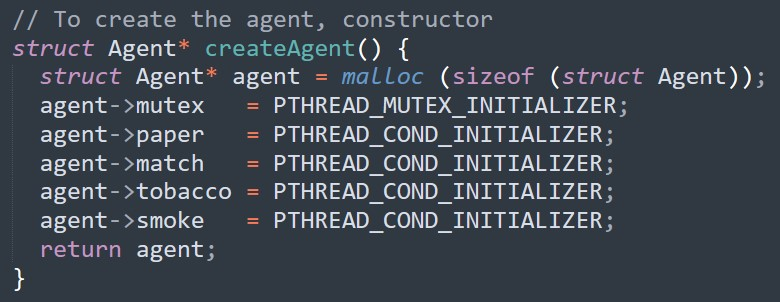
\includegraphics[width=9cm]{cs1.jpg}
\end{center}
\end{frame}
\begin{frame}{Code Snippets CV (2)}
\begin{center}
    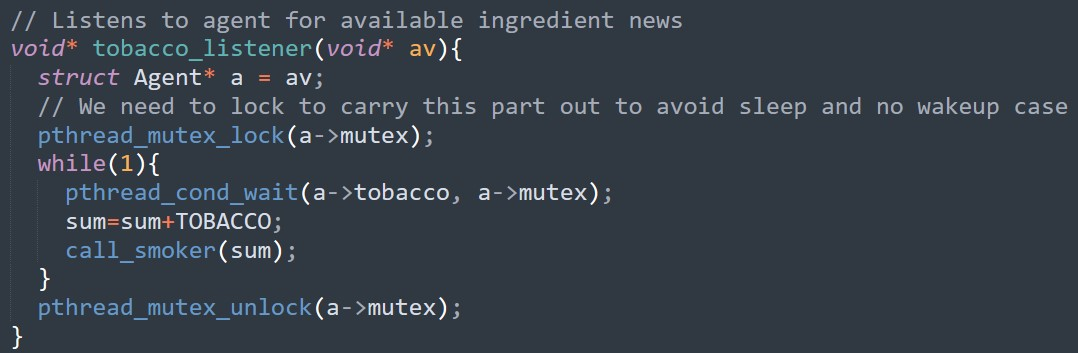
\includegraphics[width=11cm]{cs2.jpg}
\end{center}
\end{frame}
\begin{frame}{Code Snippets CV (3)}
\begin{center}
    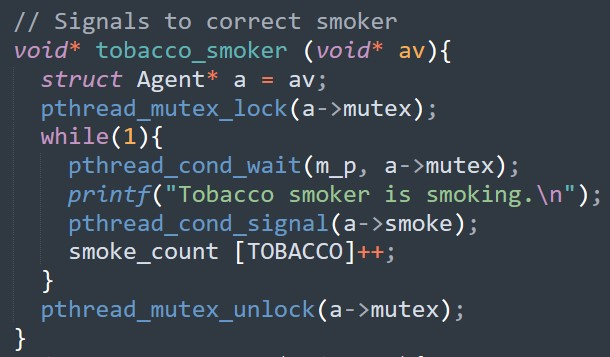
\includegraphics[width=9cm]{cs3.jpg}
\end{center}
\end{frame}

\begin{frame}{Semaphores - Working}
Here I have referred the solution provided in The Little Book of Semaphores. \\
The agent uses four semaphores, agentSem, tobSem, matSem and papSem. The first is initialized to 1 the ingredients are initialized to 0. \\
Three concurrent threads run to simulate the agent, all of them wait on the agent thread. \\
Next the issue arises that if one semaphore is updated, it is not necessary that the other ingredient on the table is also needed by a selected smoker. We need both ingredients to be the ones the smoker doesn't have. \\
For this we need three pusher codes to check if both the ingredients are indeed available
\end{frame}

\begin{frame}
\begin{center}
    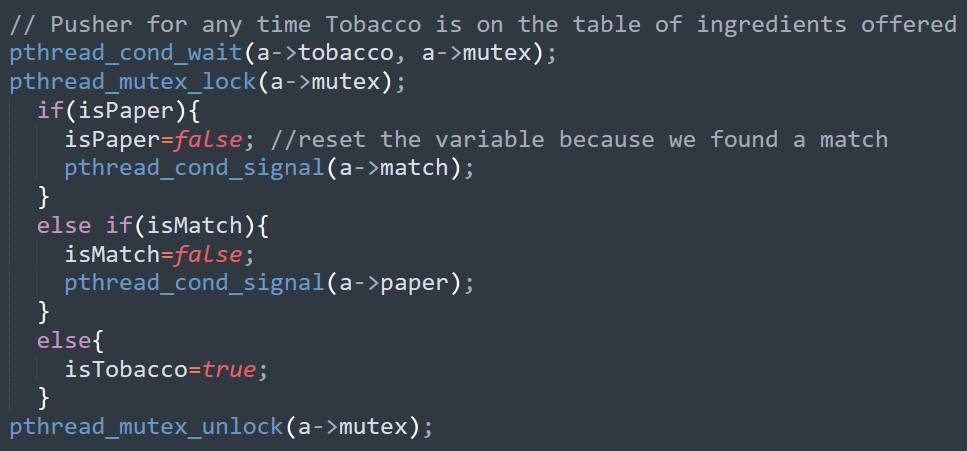
\includegraphics[width=9cm]{cs4.jpg}
\end{center}
\end{frame}

\begin{frame}{Wrong Implementation}
Wrong implementation technique for both condition variable and semaphore implementation involves the same idea. \\
Take for example a thread simulating the smoker with tobacco. He is waiting on both paper and matches. If each of the smokers had their logic as:
\begin{tcolorbox}
papSem.wait()\\
matSem.wait()\\
agentSem.signal()\\
\end{tcolorbox}
\end{frame}

\begin{frame}
Then the following deadlock could arise:\\
Suppose tobacco and paper is on the table. The matches smoker is waiting on both tobacco and paper, so seeing tobacco it gets unblocked. However, it is also likely that the tobacco smoker was waiting on paper and gets unblocked as well. This causes the first smoker to block on paper even though paper is available, and results in a deadlock. 
\end{frame}

\begin{frame}
\centering
Thank you\footnote{\tiny{Sorry for the brevity of the presentation, I started the assignment too late to do it satisfactorily}}

\end{frame}
\end{document}